\Lecturer{Hui Jin}
\Contributor{}
\LectureNumber{15}
\LectureDate{DATE}
\LectureTitle{CSS Codes and Steane Code}

\lstset{style=mystyle}


	\MakeScribeTop

%#############################################################
%#############################################################
%#############################################################
%#############################################################

\section{Introduction}
The Shor's 9-qubit code is a concatenation code structure: one repetition three code is used to deal with the bit flip noise and another repetition three code to deal with the phase flip noise. The concatenation creates a \([[9, 1, 3]]\) code, a code that encodes \(1\) logical qubit to \(9\) physical qubits, with distance three so that it can correct any single qubit error, including \(X, Y, \) or \(Z\).

This idea to use a concatenation code that an inner code deals with bit flip errors and an outer code deals with phase flip errors can be generalized. In this section, we describe a new class of quantum error-correction codes referred to as the Calderbank–Shor–Steane (CSS) codes. The construction of CSS codes is based on the use of two classical linear block codes \(C_1\) and \(C_2\). CSS code have the capability of correcting up to \(t\) bit-flip and phase-flip qubit errors, if \(C_1\) and \(C_2\) can correct \(t\) classical bit errors. But there is a caveat: not every pair of classical codes \(C_1, C_2\) can be used in a CSS construction. A necessary condition for the CSS code is the dual code of \(C_2\), namely \(C_2^{\perp}\) should be a sub-code of \(C_1\), or \(C_2^{\perp} \in C_1\). Note that this also implies that \(C_1^{\perp} \in C_2\), so at least \(C_1\) and \(C_2\) are symmetric. We will see in the next chapter why we have this requirement, using the formalization of stabilizer codes. In this chapter, we will just show that this construction works.  


I will take a top down approach in this chapter. After reviewing some of the basic results in block linear codes, we will first describe the general results of the CSS codes. Then we focus on an important instance of the CSS code, the Hadamard–Steane code, to illustrate some of the subtle details and describe how to implement the Steane code in quantum circuits. 


\section{Review of Linear Codes}
\subsection{Generator Matrix and Parity Check Matrix}
A \((n,k)\) binary linear code is generated by a basis of \(k\) vectors. It can be compactly defined either by its generator matrix or parity check matrix:  
\begin{enumerate}
    \item A generator matrix \(G\), of dimension \(n \times k\). We encode a \(k\)-bit information vector \(m\) to a \(n\)-bit codeword \(x\) by \(x = Gm\);
    \item A parity-check matrix \(H\), of dimension \(((n-k) \times n\), which satisfies \(Hx = 0\) for all codewords \(x \in C\).
\end{enumerate}
The column vector of \(G\) defines the a subspace of dimension \(k\), which produces the \(2^k\) codewords. The parity check matrix \(H\) is the null space of the subspace spanned by \(G\). That means, the row vectors of \(H\) are all orthogonal to the subspace of \(G\), or equivalently \(HG = 0\). 

We can obtain \(H\) easily from \(G\). If we write \(G\) in the systematic form,  
$$G = \begin{bmatrix}
    I_{k} \\
    P_{(n-k)\times k}
    \end{bmatrix},
$$
then the parity check matrix is:
\[H = [P_{(n-k)\times k} \; I_{n-k}].\] It is easy to see \(HG = P_{(n-k)\times k} + P_{(n-k)\times k} = 0\). That means for a codeword \(x= Gm\), we have \(Hx = HGm = 0\). 

\subsection{Dual Code}
We can define a dual code of \(C\), denoted by \(C^{\perp}\) by swapping the role of generator matrix \(G\) and parity check matrix \(H\) of the code \(C\). That is, we define a code with generator matrix \(G_{dual} = H^T\), where \(H^T\) is the transpose of \(H\). \(H^T\) has dimension \(n \times (n-k)\), therefore the encoding \(x = G_{dual} m\) encodes a \((n-k)\)-bit vector to \(n\)-bit codeword. There are \(2^{n-k}\) codewords. The parity check matrix of the dual code \(H_{dual}\) is \(G^T\). Note that the dual of \(C^{\perp}\) is \(C\). Note also that every codeword in \(C^{\perp}\) is perpendicular to every codeword in \(C\). An alternative definition of the dual code \(C^{\perp}\) is
\begin{align*}
C^{\perp} = \{b: b\cdot c = 0, \text{ for every } c in C\}. 
\end{align*}


The following lemma - Identity for linear codes and their duals - will be used later in deriving the decoding capability of CSS codes. 

\begin{lemma}
    Consider a \((n,k)\) linear code \(C\), for a \(n\)-bit vector \(z\), we have  
    \[
     \sum_{y \in C} (-1)^{y \cdot z} =
     \begin{cases}
    |C|, & \text{if } z \in C^{\perp} \\
    0.  & \text{otherwise}
    \end{cases}
    \]
\label{lemma:IdentityDual}
\end{lemma}

\begin{proof}
    If \(z \in C^{\perp}\), then \(y \cdot z = 0\) for any \(y \in C\), so \(S(z) = \sum_{y \in C} (-1)^0 = |C|. \)

    Now consider the non-trial case \(z \notin C^{\perp}\). We know the codespace \(C\) is an abelian group.  The dot product \(\phi_z(y) = y\cdot z\) is a group homomorphism\footnote{The function \(h : G(\star) \rightarrow H(\cdot)\) is a group homomorphism if whenever
\(a \star b = c\)  we have   \(h(a) \cdot h(b) = h(c).\)
In other words, the group H in some sense has a similar algebraic structure as G and the homomorphism h preserves that.
}: \(C \rightarrow Z_2\). This map is surjective when \(z \notin C^{\perp}\), which means that \(K = kernel(\phi_z(y))\) is an index two  subgroup of \(C\). The two cosets - one mapping to \(0\), the other mapping to \(1\) - have the same size. (Another way to see this is that given an element \(s \in C\) where \(\phi_z(s) = 1\), we have for any \(y \in C\) if and only \(\phi_z(y) = 0\) then \(\phi_z(y + s) = 1\), which means the whole set of codewords can be partitioned into two equal size sets whose elements are mapped to \(0\) and \(1\) respectively.) Therefore \(|K|=|C|/2\) and the result follows.

    Alternatively, the non-trial trial case \(z \notin C^{\perp}\) can be explained as the following.

    Assume \(c_0\) is one codeword in \(C\) such that \(c_0 \cdot z = 1\). Then if \(c_1\cdot z = 0\), we have \((c_0 + c_1)\cdot z = 1\);
    if \(c_1\cdot z = 1\), we have \((c_0 + c_1)\cdot z = 0\). That means the whole codewords is partitioned into two groups of equal size such that one group has \(c\cdot z = 0\) and the other group \(c \cdot z =1\) and the result follows.
    This is basically the plain language explanation of the homomorphism proof.
\end{proof}


\section{The Noise Model}
We have seen the bit-flip noise and phase-flip noise in the introduction of the quantum noise. Here we use a more compact notation. For a \(n\)-qubit \(\ket{x}\), the bit-flip noise and phase bit noise can be modeled as a bit vector \(e_X\) and \(e_Z\), such that the distorted \(n\)-qubit \(\ket{x^{\star}}\) is 
\begin{equation}
    \ket{x^{\star}} = (-1)^{x\cdot e_Z} \ket{x+e_X} \label{eq:QEC_noise}
\end{equation}
where \(x \cdot e_Z\) is the dot product of \(x\) and \(e_Z\). We use \(e_X\) to indicate the error is caused by Pauli matrix \(X\), and \(e_Z\) to indicate the error is caused by Pauli matrix \(Z\). 

For instance, \(\ket{x} = \ket{10011}, e_X = (0, 1, 0, 1, 0) \) and \(e_Z = (1, 0, 0, 1, 1)\) yield \(x \cdot eZ = 3\)  and \(x+e_X = 11001\), and the distorted state \(\ket{x^{\star}} = (-1)^3 \ket{11001} = - \ket{11001}\).

\section{Quantum Hamming Bound}
A t-error correcting quantum code is defined to be a code for which all errors of weight less than or equal to t are correctable. Since there are 3 possible single-qubit errors, the number of error operators of weight t acting on n qubits is 3tC(n,t). Therefore a t-error correcting code must be able to correct Pti=0 3iC(n,i) error operators. For nondegenerate codes, ⟨u|E1E2 |u⟩ = 0 in (31), every codeword |u⟩ and all its erroneous versions M |u⟩ must be orthogonal to every other codeword and all its erroneous versions. All these orthogonal states can only fit into the 2n-dimensional Hilbert space of n qubits if
\begin{align*}
    |C| \sum_{i=0}{t} 3^i \binom{n}{i} &\leq 2^n \\
\end{align*}
This bound is known as the quantum Hamming bound. For large \(n, t\), it becomes 
\begin{align*}
    R = k/n \leq 1 - \frac{t}{n} \log_2 3 - H(\frac{t}{n}).\\
\end{align*}
Let us plot this figure. The rate \(k/n\) falls to zero at \(\frac{t}{n} \approx 0.189\). 

Quantum Hamming bound is an upper bound. We also can derive a similar lower bound as Gilbert-Varshamov in the classical coding theory. 

\section{CSS Code}
The basic idea of CSS codes is to use a concatenation of two classical codes \(C_1\) and \(C_2\) that one is used to deal with bit flip noise and the other to deal with the phase flip noise. There is restriction on the structure of \(C_1\) and \(C_2\) to ensure that they indeed work together. 


To construct a CSS code, we require the following two conditions:
\begin{enumerate}
    \item All codewords of \(C_2^{\perp}\) belong to \(C_1\), or \(C_2^{\perp} \in C_1\); 
    \item \(C_1\) and \(C_2\) can correct \(t\) bit errors.
\end{enumerate}

Condition 1) seems hard to grasp initially. First, there seems an asymmetry present between \(C_1\) and \(C_2\).  Fortunately, it is trivial to check \(C_2^{\perp} \in C_1\) is equivalent to \(C_1^{\perp} \in C_2\) so \(C_1\) and \(C_2\) are symmetric. 

To truly understand where this condition comes from, we need to use the formalization of stabilizer codes, which we will introduce in the next chapter. For now, we will show codes with such constraints indeed work, with a touch of mystery. 

We will define codewords using the concept of cosets. So let us define that first. 

\subsection{Coset}
Given a group \(A\) and its subgroup \(B\), and its associated operator \(+\), we can define the coset of any element \(a \in A\) with respect to \(B\) as a set of elements generated by a translation of the elements in \(B\) using \(a\):
\begin{align*}
Coset(a) = \{a + b \;|\; b \in B\}.
\end{align*}
Each coset has \(|B|\) elements. Since \(B\) is a subgrop of \(A\), we have the following property:
\begin{theorem}
    For any \(x, y \in A\), either \( Coset(x)\) is identical to \(Coset(y)\), or \(Coset(x)\) does not overlap with \(Coset(y).\)
\end{theorem}

\begin{proof}
The statement is equivalent  to if \(Coset(x)\) and \(Coset(y)\) has at least one common element, then they must be identical. Let us assume \(x+b_1 = y + b_2\) is the common element, where \(x+b_1\in coset(x)\) and \(y+b_2\in coset(y)\). That means \(y-x = b_1 - b_2 \in B\) as \(b_1, b_2 \in B\). Denote \(d = y-x\). Then \(Coset(y) = \{y + b \;|\; b \in B\} = \{x + d + b \;| \;b \in B\} = {x + b' | b' \in B} = Coset(x).\)
\end{proof}

\begin{corollary}
The total number of distinct cosets is 
\[\frac{|A|}{|B|}.\]
\end{corollary}
\begin{proof}
Every element of \(A\) is in one and only one of the cosets; each coset has \(|B|\) elements which are all elements in \(A\). Therefore, there are \(\frac{|A|}{|B|}\) distinct cosets. 
\end{proof}

\subsection{Codeword Definition}
Given two linear block codes \(C_1, C_2\) satisfying the above conditions, we can construct a CSS code as follows.   First we define a quantum state \(\ket{x + y}\), for a pair of two n-bit vectors \(x, y\), where \(+\) indicates here bit-wise addition modulo \(2\). For instance, if \(x = 00101\) and \(y = 10111\), we have \(\ket{x + y} = \ket{10010}\). Now given \(x \in C_1\), we construct the the quantum state \(\ket{x + C_2^{\perp}}\) as the superposition of the Coset(x): 
\begin{align}
\ket{x + C_2^{\perp}} = \frac{1}{\sqrt{|C_2^{\perp}|}}\sum_{y \in C_2^{\perp}} \ket{x+y}.
\label{eq:QEC_CSS1}
\end{align}
The quantum state \(\ket{x + C_2^{\perp}}\) is a one-to-one map to the \(Coset(x)\); in fact, the quantum state \(\ket{x + C_2^{\perp}}\) is the normalized sum of the bases \(\ket{x+b\;|\; b \in C_2^{\perp}}\).


When the error pattern \(e_X, e_Z\) is applied to the CSS codeword \(\ket{x + C2^{\perp}}\) defined in Eq.~\ref{eq:QEC_CSS1}, the resulting distorted state is
\begin{align}
\ket{(x + C_2^{\perp})^{\star}} = \frac{1}{\sqrt{|C_2^{\perp}|}}\sum_{y \in C_2^{\perp}} (-1)^{(x+y)\cdot e_Z} \ket{x+y + e_X}.
\label{eq:QEC_CodeNoisy}
\end{align}

\subsection{Detect and Correct bit-flip noise \(e_X\)}
The first step in decoding consists of the introduction of the parity-check matrix \(H\) to correct \(e_X\). 

This is achieved by appending an n-qubit ancilla \(\ket{0}\) to \(\ket{x^{*}} = \ket{x + y + e_X}\), and passing the result through a quantum circuit that achieves the transformation \
\begin{align}
    \ket{x^{*}}\ket{0} &\rightarrow \ket{x^{*}}\ket{H x^{*}}  \label{eq:QEC_BEC} \\ 
    &= \ket{x^{*}}\ket{H(x+y) + H e_X}\nonumber\\
    &= \ket{x^{*}}\ket{H e_X}.  \nonumber 
\end{align} 
In the last step \(H(x+y)=0\) because both \(x, y\) are codewords in \(C_1\).  

The details of the quantum circuit will be describe in the Steane code example in the next section. 

Measuring each of the qubits in the ancilla \(\ket{H e_X}\) yields the syndrome vector \(H e_X\), which is common to each of the series terms in Eq.~(\ref{eq:QEC_CodeNoisy}). So the ancilla qubits are disentangled from the original qubits and can be measured without disturbing the original qubits. This syndrome measurement \(\ket{H e_X}\) will determine the error (albeit with high complexity as we are assuming here a general syndrome decoder.)
Given the error correction capability of \(C_1\), it is guaranteed that any \(t\)-error can be corrected by applying X gates in the corresponding circuit wires, the distorted \(n\)-qubit in Eq~(\ref{eq:QEC_noise}) becomes
\begin{align*}
       \ket{x^{\star}} = (-1)^{x\cdot e_Z} \ket{x}. 
\end{align*}
Therefore, the distorted state of a CSS codeword no long has the bit flip noise and gets a little cleaner, and becomes:  
\begin{align}
\ket{(x + C_2^{\perp})^{\star}}_{X} = \frac{1}{\sqrt{|C_2^{\perp}|}}\sum_{y \in C_2^{\perp}} (-1)^{(x+y)\cdot e_Z} \ket{x+y}.
\label{eq:QEC_CSSII}
\end{align}


\subsection{Detect and Correct phase-flip noise \(e_Z\)}
To correct the phase flip noise, we will first pass the X-corrected state \(\ket{(x + C_2^{\perp})^{\star}}_{X}\) through the Hadamard gate \(H^{\otimes n}\), and we get 
\begin{align}
    H^{\otimes n} \ket{(x + C_2^{\perp})^{\star}}_{X} &= \frac{1}{\sqrt{|C_2^{\perp}|}}\sum_{y \in C_2^{\perp}}  (-1)^{(x+y)\cdot e_Z} H^{\otimes n} \ket{x+y} \nonumber \\
    &= \frac{1}{\sqrt{|C_2^{\perp}|2^n}}\sum_{y \in C_2^{\perp}} (-1)^{(x+y)\cdot e_Z} \sum_{k=0}^{2^n-1} (-1)^{(x+y)\cdot k} \ket{k} \nonumber\\
    &= \frac{1}{\sqrt{|C_2^{\perp}|2^n}}\sum_{y \in C_2^{\perp}}\sum_{k=0}^{2^n-1}(-1)^{(x+y)\cdot (e_Z + k)}\ket{k} \nonumber\\
    &= \frac{1}{\sqrt{|C_2^{\perp}|2^n}}\sum_{y \in C_2^{\perp}}\sum_{k'=0}^{2^n-1}(-1)^{(x+y)\cdot k'}\ket{k' + e_Z} \nonumber\\
    &= \frac{1}{\sqrt{|C_2^{\perp}|2^n}}\sum_{k'=0}^{2^n-1}(-1)^{x\cdot k'}(\sum_{y \in C_2^{\perp}}(-1)^{y\cdot k'})\ket{k' + e_Z}\label{eq:QEC_PE}
\end{align}

By Lemma~\ref{lemma:IdentityDual}, with \(C_2\) and \(C_2^{\perp}\) swapped, we have 
\[
\sum_{y \in C_2^{\perp}}(-1)^{y\cdot k'} = 
\begin{cases}
    |C_2^{\perp}|, & \text{if } k' \in C_2\\
    0, & \text{otherwise}
\end{cases}
\]
Therefore in Eq.~(\ref{eq:QEC_PE}) the sum over \(k'\) has non-zero term if and only if  \(k' \in C_2\), so the sum  becomes 
\begin{align}
H^{\otimes n} \ket{(x + C_2^{\perp})^{\star}}_{X} &= \frac{1}{\sqrt{|C_2^{\perp}|2^n}}\sum_{k'=0}^{2^n-1}(-1)^{x\cdot k'}(\sum_{y \in C_2^{\perp}}(-1)^{y\cdot k'})\ket{k' + e_Z} \nonumber \\
&= \frac{1}{\sqrt{|C_2^{\perp}|2^n}}\sum_{k'\in C_2}(-1)^{x\cdot k'} |C_2^{\perp}| \ket{k' + e_Z} \nonumber\\
&= \sqrt{\frac{|C_2^{\perp}|}{2^n}}\sum_{k'\in C_2}(-1)^{x\cdot k'} \ket{k' + e_Z} \label{eq:QEC_PEC}
\end{align}

At this point, we effectively turned the phase flip error to a bit flip error. The use of Hadamard matrix to achieving this is in principle the same as in the Shor's 9-bit code. Now we can use the same technique as in Eq.~\ref{eq:QEC_BEC}, to correct the error \(e_Z\), by using the parity check matrix of code \(C_2\) to obtain the syndrome. By construction, \(C_2\) can correct \(t\) errors. 

After correction, we obtain
\begin{align*}
\sqrt{\frac{|C_2^{\perp}|}{2^n}}\sum_{k'\in C_2}(-1)^{x\cdot k'} \ket{k'}, 
\end{align*}
which corresponds to the Hadamard transform of the original codeword: \[H^{\otimes n} \ket{(x + C_2^{\perp})}.\]
Applying Hadamard transformation again inverts back to the original codeword \(\ket{(x + C_2^{\perp})}\). 

\section{Steane Code}
In this section, we describe an important instance of a CSS code, the Steane code. It is based on our familiar Hamming code \(C_1 = (7, 4)\), and its dual \(C_2 = C^{\perp}\). 


The Steane code has the same bit-flip and phase-flip error correction capability as the earlier-described Shor 9-bit repetition code, namely, up to one error in either or both cases, but it uses \(7\)-qubit codewords, thus more efficient than the Shor's code. The best code to achieve the same capability uses \(5\)-qubit. 

\subsection{The definition of \(C_1\) and \(C_2\)}

\(C_1\) is the \(7,4,3)\) Hamming code. It is able to correct \(1\) (classical) bit error. The generator matrix \(G\) of \(C_1\) is: 
$$G = \begin{bmatrix}
    1 & 0 & 0 & 0\\
    0 & 1 & 0 & 0\\
    0 & 0 & 1 & 0\\
    0 & 0 & 0 & 1\\
    0 & 1 & 1 & 1\\
    1 & 0 & 1 & 1\\
    1 & 1 & 0 & 1
\end{bmatrix}$$
A codeword in \(C_1\) is generated by \(c = Gm\), where message \(m\) is a length-4 column vector.

The corresponding parity check matrix \(H\) of \(C_1\) is:  
$$H = \begin{bmatrix}
    0 & 0 & 0 & 1 & 1 & 1 & 1\\
    0 & 1 & 1 & 0 & 0 & 1 & 1\\
    1 & 0 & 1 & 0 & 1 & 0 & 1
\end{bmatrix}$$
where a length-7 column vector \(c\) is a codeword iff \(Hc= 0.\) By construction, \(HG=0\), ie the row vectors of \(H\) defines the null space of the subspace defined by the column vectors of \(G\).


\(C_2\) is the dual code of \(C_1\). A dual code of \(C_1\) simply means that we use the transpose of parity check matrix \(H^T\) of \(C_1\) as the generator matrix of \(C_2\):
$$G_{dual} = \begin{bmatrix}
    0 & 0 & 1\\
    0 & 1 & 0\\
    0 & 1 & 1\\
    1 & 0 & 0\\
    1 & 0 & 1\\
    1 & 1 & 0\\
    1 & 1 & 1
\end{bmatrix}$$
A codeword in \(C_2\) is generated by \(c = G_{dual} m\), where message \(m\) is a length-3 column vector. 


\begin{lemma}
    All codewords in \(C_2\) belong to \(C_1\). 
\end{lemma}

\begin{proof}
We will show that any codeword \(c\) in \(C_2\) is also in \(C_1\) by showing \(Hc = 0\). A codeword \(c\) in \(C_2\) can be written as \(c = G_{dual} m = H^T m\). Therefore \(Hc = H H^T m\). Notice that the row vectors of \(H\) are orthogonal to each other, so \(H H^T = 0\) and the results follows. 
\end{proof}

Now since \(C_2\) is the dual of \(C_1\), the dual of \(C_2\) is \(C_1\), ie. \(C_2^{\perp} = C_1\).

Thus, based on the construction, \(C_1\) and \(C_2\) has the following property: 

\begin{enumerate}
    \item All codewords of \(C_2\) belong to \(C_1\); 
    \item \(C_1\) and \(C_2^{\perp}\) are the same \((7,4,3)\) Hamming code, which can correct \(1\) bit error.
\end{enumerate}

So the Steane code satisfies the conditions specified in the CSS code requirement and is able to correct bit flip and/or phase flip on a single bit. 

\subsection{A Compact way to represent the codewords of \(C_2\)}
The parity check matrix of \(C_2\) is \(H_{dual} = G^T\):
$$H_{dual} = \begin{bmatrix}
    1 & 0 & 0 & 0 & 0 & 1 & 1 \\
    0 & 1 & 0 & 0 & 1 & 0 & 1 \\
    0 & 0 & 1 & 0 & 1 & 1 & 0 \\
    0 & 0 & 0 & 1 & 1 & 1 & 1
\end{bmatrix}$$
Based on this, the parity bits based the three message bits \(m_1, m_2, m_3\) are 
\begin{align*}
    p_1 &= m_2 + m_3 \\
    p_2 &= m_1 + m_3 \\
    p_3 &= m_1 + m_2 \\
    p_4 &= m_1 + m_2 + m_3 
\end{align*}
Thus three messages bits \(m_1, m_2, m_3\) is encoded to 
\begin{align}
code(m_1, m_2, m_3) = (m_2 + m_3, m_1 + m_3, m_1 + m_2, m_1 + m_2 + m_3, m_1, m_2, m_3)
\label{eq:QEC_HammingDualEncode}
\end{align}

We can list the 8 codewords: 
\begin{align*}
    0000000,  1101001, & 1011010, 0110011 \\
    0111100,  1010101, & 1100110, 0001111 \\
\end{align*}

\subsection{The Steane Codeword}
There are \(\frac{|C_1|}{|C_2|} = \frac{2^4}{2^3} = 2\) codewords in the Steane code. They are the two following cosets, denoted by logit qubits \(\ket{\hat{0}}\), and \(\ket{\hat{1}}\):
\begin{align*}
    \ket{\hat{0}} &= \ket{0000000 + C_2} \\
    \ket{\hat{1}} &= \ket{1111111 + C_2}  
\end{align*}
Expanding the above codeword into bases, and using the fact how the codewords are generated from the message bits Eq.~(\ref{eq:QEC_HammingDualEncode}), we have 
\begin{align}
\ket{\hat{0}} &= \ket{0000000 + C_2} \nonumber\\
&\defeq \frac{1}{\sqrt{8}}\sum_{c\in C_2}\ket{0000000 + c} \nonumber\\
&= \frac{1}{\sqrt{8}} (\ket{0000000} + \ket{1101001} + \ket{1011010} + \ket{0110011} + \nonumber \\ 
 &\;\;\;\;\;\;\;\;\;\;\ket{0111100}  + \ket{1010101}  + \ket{1100110} + \ket{0001111}) \nonumber \\
 &= \frac{1}{\sqrt{8}} \sum_{m_1,m_2,m_3}\ket{m_2 + m_3}\ket{m_1 + m_3}\ket{m_1 + m_2} \ket{m_1 + m_2 + m_3}\ket{m_1}\ket{m_2}\ket{m_3} \label{eq:QEC_SteaneSum1}
\end{align}

Similarly, 
\begin{align}
\ket{\hat{1}} &=  \ket{111111 + C_2} \nonumber\\
  &=\frac{1}{\sqrt{8}}\sum_{m_1,m_2,m_3}\ket{m_2 + m_3+1}\ket{m_1 + m_3 + 1}\ket{m_1 + m_2+1} \otimes \nonumber\\
   & \;\;\;\;\;\;\;\;\;\ket{m_1 + m_2 + m_3+1} \ket{m_1+1}\ket{m_2+1}\ket{m_3+1} \nonumber\\
   &= \frac{1}{\sqrt{8}} \sum_{m_1^{'},m_2^{'},m_3^{'}}\ket{m_2^{'} + m_3^{'}+1}\ket{m_1^{'} + m_3^{'} + 1}\ket{m_1^{'} + m_2^{'}+1} \otimes \nonumber\\
   &\;\;\;\;\;\;\;\;\;\ket{m_1^{'} + m_2^{'} + m_3^{'}} \ket{m_1^{'}}\ket{m_2^{'}}\ket{m_3^{'}} \label{eq:QEC_SteaneSum2}
\end{align}
We replace \(m_i + 1\) by \(m_i^{'}\) in the last step.  

The Eqs~(\ref{eq:QEC_SteaneSum1}) and (\ref{eq:QEC_SteaneSum2}) can be combined to one encoding logic for logit qubit \(\ket{a}\): 
\begin{align}
\ket{\hat{a}} &=\frac{1}{\sqrt{8}} \sum_{m_1,m_2,m_3}\ket{m_2 + m_3+a}\ket{m_1 + m_3 + a}\ket{m_1 + m_2+a} \ket{m_1 + m_2 + m_3} \ket{m_1}\ket{m_2}\ket{m_3} \label{eq:QEC_SteaneSum}     
\end{align}


\subsection{The Quantum Circuit for the Steane Code}

The key element in the quantum circuit to implement the Steane code is how to realize the summation in Eq.~(\ref{eq:QEC_SteaneSum}). 

Our powerful Hadamard transforms does something similar to Eq~\ref{eq:QEC_SteaneSum1} already,  
\[H^{\otimes 3}\ket{0}^{\otimes 3} =\frac{1}{\sqrt{2^3}} 
\sum_{m_1,m_2, m_3} \ket{m_1}\ket{m_2}\ket{m_3}.\]
What we are missing are the qubits corresponding to the parity bits. How do we get these? 

Let us analyze an elementary circuit in  Figure~\ref{fig:QEC_SteaneSimple}.
 
 \begin{figure}[h]
    \centering
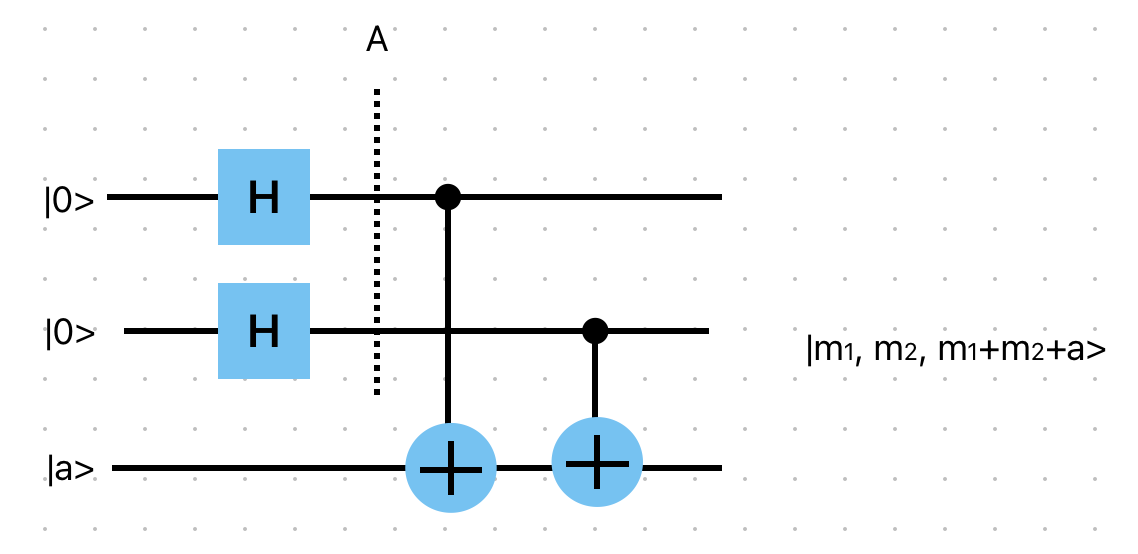
\includegraphics[width=0.6\textwidth]{Figs/Steane_simple.png}
    \caption{An elementary circuit to generate a code with a simple parity.}
    \label{fig:QEC_SteaneSimple}
\end{figure}

It is seen from the figure that the two Hadamard gates produce \(\ket{+}^{\otimes 2}\) at the place indicated by "A", which is \[\sum_{m_1,m_2} \ket{m_1}\ket{m_2} = \frac{1}{2}(\ket{00} + \ket{01} + \ket{10}+ \ket{11}.\] They act as control qubits on the target qubit \(\ket{a}\)  through CNOT gates. This circuit generate a simple code where logic qubit \(\ket{a}\) is mapped to the codeword: 
\[\frac{1}{2} 
\sum_{m_1,m_2} \ket{m_1}\ket{m_2}\ket{m_1+m_2+a}.\]


We first observe that \(\ket{a}\), which represents the originator’s message qubit to be encoded, is not limited to the basis states \(\ket{0}\) or \(\ket{1}\); rather, by linearity, the encoding also works for general qubit \(\ket{a} = \alpha\ket{0} + \beta\ket{1}\).

Based on the same principle, we can draw the quantum circuit to generate the Steane code as the sum in Eq.~(\ref{eq:QEC_SteaneSum}). 

 \begin{figure}[h]
    \centering
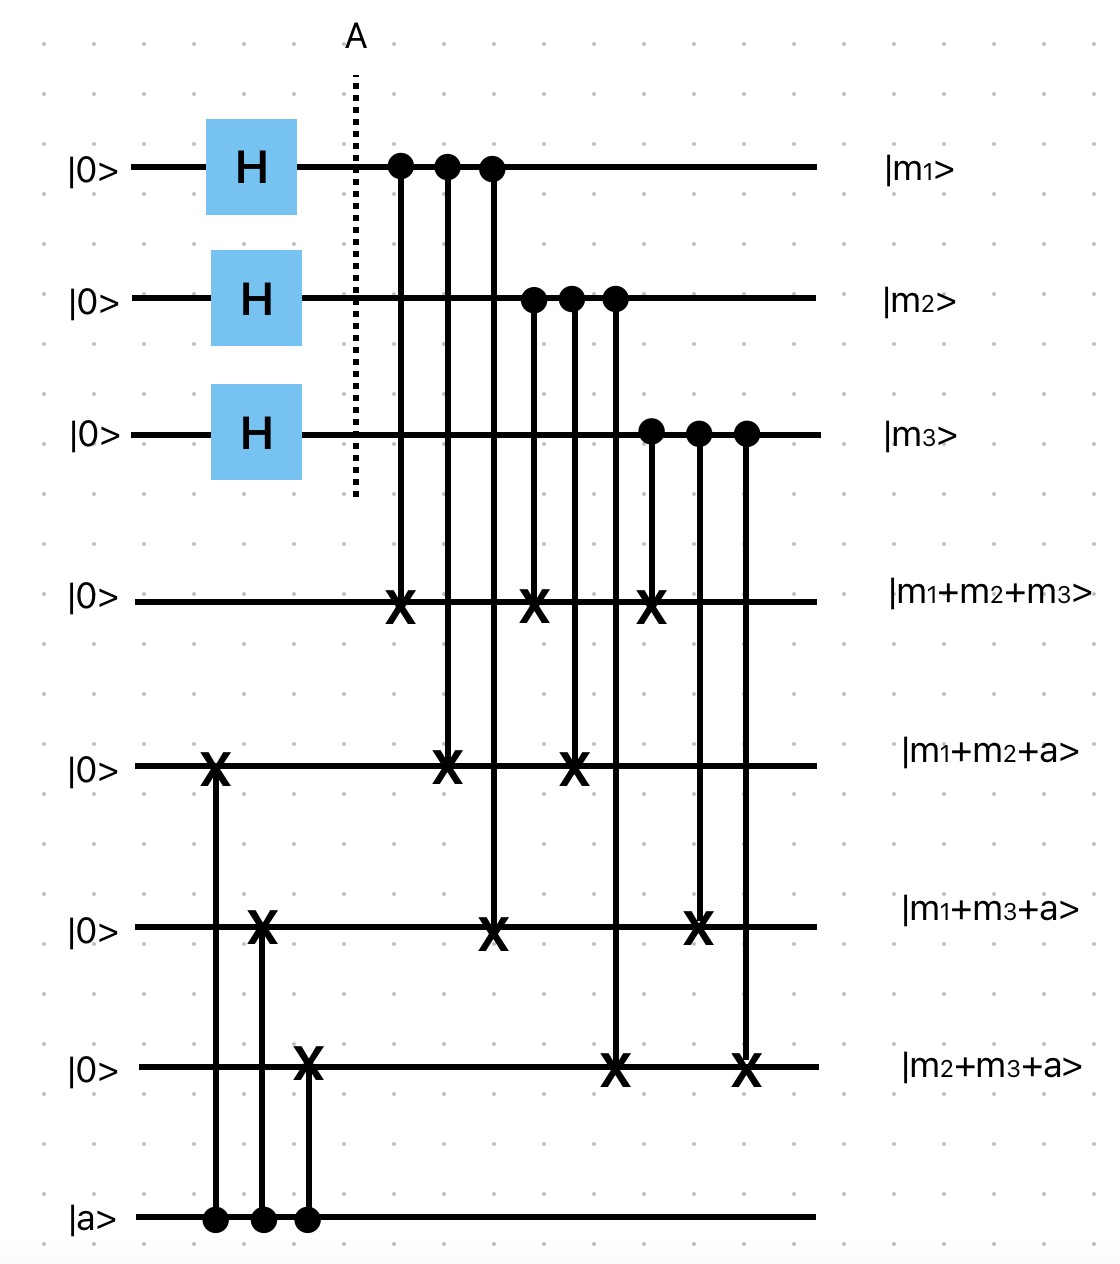
\includegraphics[width=0.7\textwidth]{Figs/Steane_FullCode.png}
    \caption{The quantum circuit to realize Steane code.}
    \label{fig:QEC_SteaneFullCode}
\end{figure}


\section{Intuition on Syndrome Extraction}
The syndrome extraction operation is
\begin{align}
XOR^{(H)}_{q,a}(\ket{0}_a \ket{u+e})= \ket{H eT}_a \ket{u+e} 
\end{align}
The fact that the classical syndrome is independent of the message is now highly significant, for if the initial state of q is any superposition \(\sum_{u in C} a_u \ket{u}\), the syndrome extraction does not leave \(q\) and \(a\) entangled:
\begin{align*}
XOR^{(H)}_{q,a}(\ket{0}_a X_e \sum_{u in C} a_u \ket{u} =\ket{H eT}_a \sum_{u \in C} a_u \ket{u+e}
\end{align*}
Recovery is completed by measuring \(a\), deducing \(e\) from \(HeT\), and applying \(X_e\) to \(q\).

\section{Exercises}
\begin{enumerate}
    \item Prove the dual code theorem. 
    \begin{align*}
        H^{\otimes n} \sum_{i \in C} \ket{i} = \sum_{i \in C^{\perp}} \ket{i}.
    \end{align*}
\end{enumerate}